%
%   F U J I W A R A
%   "kfuji.tex"
%

\documentclass[10pt,b5paper,papersize,dvipdfmx]{jsbook}

\usepackage{vuccaken}
\usepackage{vuccaken2019}

% スタイルファイルの読み込みや自作マクロは、
% 最終的には vuccaken2019.sty の中に書いてください。
% とりあえずはここに書いてもらって構いません。


\begin{document} % 以下本文

\mokuji{2} % 目次出力

% - - - - - - - - - - - - - - - - - - - - - - - - %
\kaishititle%
  {Python入門}% title
  {理工学部機械工学科1回生}% 所属
  {\vname{藤原}{弘貴}}% name
% - - - - - - - - - - - - - - - - - - - - - - - - %

%
\section*{はじめに}
今年度の9月から本格的にpythonと言うよりプログラミング自体を学び始めたのですが、基礎の学習が終わり環境構築もひと段落ついたので一度まとめてみようと思いました。プログラミングって何?pythonに興味があるって言う人はぜひ読んでいただけると幸いです。\par
因みに少しでも犠牲者を減らしたいのですが、機械工学科では名前の通り機械(ロボット)をメインで扱うのではなく、4力という材料力学、流体力学、熱力学、機械力学といったものを扱います。プログラミングや物理学などをメインとして学びたい場合は他学科をお勧めします。どんな研究室があるか大学のサイトで確認してみると良いです。\par
%
\clearpage

\section{本誌の対象と目標}
\subsection{対象}
pythonがそもそも何なのか知らない人から文法を一通り勉強し、実際に自分のパソコンで何か作ってみたいなという人までが対象です。他にも環境構築が終わった後、実際に何をしたら良いかわからない人でも大丈夫です。\par
主にmacOSを使って解説を行いますが、やり方自体はさほど変わらないので無料のOS Linuxやwindowsの方でも参考になるかと思います。\par
\subsection{目標}
本誌での一番の目標はpythonの環境構築です。Pythonの文法に関しては説明しませんが、自分がやってみてよかったと思える学習方法は
説明したいと思います。\par
\section{Pythonとはなんなのか}
\subsection{そもそもプログラミングとは}
プログラミングと聞いて自分には無理だと思うかもしれません。
黒い画面に緑色の文字が大量に流れているようなものをイメージしている方がいるかもしれませんが、実際はそんなことはありません。
難しいことをやるとなると数学やアルゴリズムなどの知識必要になってきますが、基本的には決まった文法通りに書くことでパソコンがそれを読み取り、機械が理解できる言語に変換された後、書かれた内容その通りに実行するというだけです。
言語によって得意不得意があったり、文法が違ったりします。日本語や英語、中国語と言ったような自然言語は文法の他に単語を覚えたりしますが、プログラミング言語の場合は基本的に英語で書かれていて、文法も覚える必要はありません。
ですので、1つ理解してしまえば、2つ3つ学習するときは簡単に学習することが可能です。\par
\subsection{結局Pythonで何ができるのか}
% \begin{figure}[htbp]
%   \centering
%   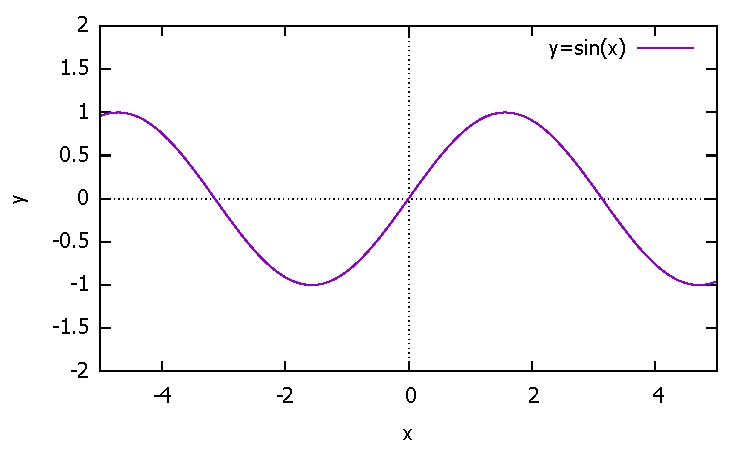
\includegraphics[width=10cm]{temp/fig-sin.pdf}
%   \caption{$y=\sin x$のグラフ。gnuplotで作成した。}
%   \label{fig:sin}
% \end{figure}

%% 参考文献
\begin{thebibliography}{99}
  \item 著者, 本やページの名前, (URL), 出版社, 出版年.
\end{thebibliography}


\end{document}
%
% ファイトだよ!
%